\section{Shashlik + Hadron Endcap} \label{section:simulations_shashlik}
The second candidate for the CMS Phase 2 upgrade was the Shashlik + Hadron Endcap. This system actually features two separate calorimeters, one for the electromagnetic component and one for the hadronic. Both rely on the scintillation process in order to measure the energy of the showers. Figure~\ref{fig:higgs_simulations_shashlikexamples} shows a custom built full CMS scale ``Shashlik + Hadron Endcap'' detector.
\begin{figure}[htbp]
    \centering
    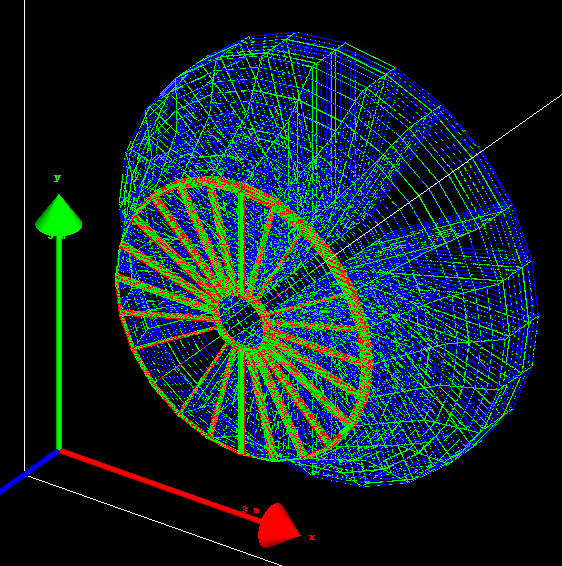
\includegraphics[width=0.9\textwidth]{figures/ch_simulations/shashlik/geometry/Shashlik+HE_Complete_Wire.png}\\
    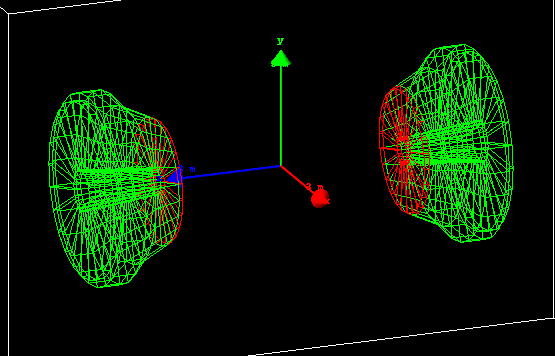
\includegraphics[width=0.9\textwidth]{figures/ch_simulations/shashlik/geometry/SHE_70_20.png}
    \caption{Full CMS Scale ``Shashlik + HE'' System (from different angles).}
    \label{fig:higgs_simulations_shashlikexamples}
 \end{figure}

\subsection{Physical Layout}
Shashlik is an Electromagnetic Calorimeter System with the name implicitly reflecting its structure and the choice of readout technology. The physical layout is similar to HGC discussed in Section~\ref{section:simulations_hgc}: alternating layers of absorber and active materials, however there is no electronics unit sitting on the calorimeter itself. Instead, wave-length shifting fibers go through the entire length of the calorimeter and are responsible for light capture and transmission to the electronics unit for conversion into an analog signal. The full specification of the Shashlik Calorimeter can be summarized as follows:
\begin{itemize}
    \item 25-30 $X_0$ device.
    \item No Longitudinal Segmentation.
    \item Alternating layers of absorber (tungsten W) and active (LYSO) materials.
    \item Active Material used is LYSO crystal scintillator.
\end{itemize}
Hadron Endcap (HE) is an active CMS Endcap Calorimeter that is part of the HCAL subsystem. Its design principles are similar with respect to Shashlik, however hadron calorimeter has a slightly different choice of readout technology \cite{Baiatian:2008zz}. The Calorimeter specification can be summarized as follows:
\begin{itemize}
    \item $10\lambda$ device.
    \item Alternating layers of absorber (Brass) and active (SCSN-81 plastic scintillator) materials \cite{Baiatian:2008zz}.
    \item Partial longitudinal segmentation.
\end{itemize}

\subsection{Detector Readout}
For the purpose of simplification, in the simulation the assumption is made to have a perfect light capture and transmission for both Shashlik and Endcap. Also no modeling of the wave-length shifting fibers or any kind of photodetectors is done. In other words, this study looks for upper limits of our calorimeter performance. The metric of the system's response is defined to be the number of generated photons within the scintillator. The scintillation mechanism is responsible for light generation and G4Scintillation \cite{geant4}; the physics process of {\sc Geant4} provides these capabilities via optical photons. For the purpose of modeling, {\sc Geant4} defines two different types of photons: regular photons, that obey the laws of quantum physics, and optical photons, that follow the laws of geometrical optics. Optical photons do not participate in the conservation of energy laws and do not deposit any energy into the scintillator (this fact allows for optimizations).

\subsection{Parametrized Detector Readout}
Typical light yields for a scintillator are in thousands of optical photons per MeV of deposited energy into the scintillation material. The exact number is material-dependent and varies substantially. Given that the input particle has energies in the GeV range, the number of optical photons that gets is goes well above 1 million. Tracing all of these photons is a complicated and time-consuming task for {\sc Geant4}'s engine. Moreover, given that optical photons can not deposit energy into the material, one can simply count and kill them right after they have been generated. Therefore, for the purpose of optimizing the time it takes to generate a single event, the parametrization of the response of a scintillator is performed. This procedure allows to substantially speed up the simulation without degrading the performance.

\subsection{Analysis and Results}
The analysis procedure is identical to the one described for HGC in Section~\ref{section:simulations_hgc} with two main differences. First, the readout metric here is defined to be simply the total number of generated optical photons. No layer by layer weighting is applied for neither Shashlik nor HE. And second, the HE is calibrated separately, by shooting pions with a different set of energies. Figure \ref{fig:simulations_shashlik_linearity} shows the results of computing the linearity for both Shashlik and HE. It is clear, especially comparing to {\sc HGC}, that Shashlik exhibits better linearity properties. The yield per $1$ GeV is about $5.3$ $\times$ $10^6$ for Shashlik and $7.0$ $\times$ $10^4$ for Hadron Endcap.
 \begin{figure}[htbp]
    \centering
    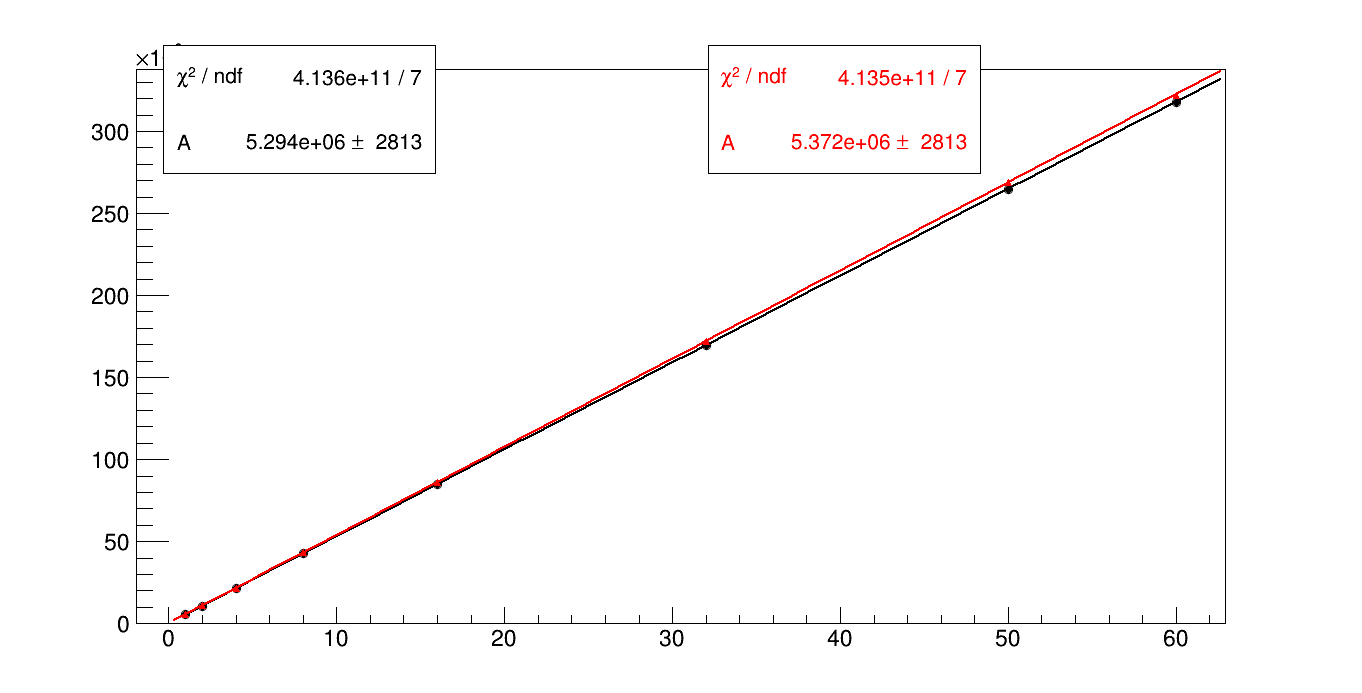
\includegraphics[width=0.95\textwidth]{figures/ch_simulations/shashlik/performance/ResponseVsEnergy.png}\\
    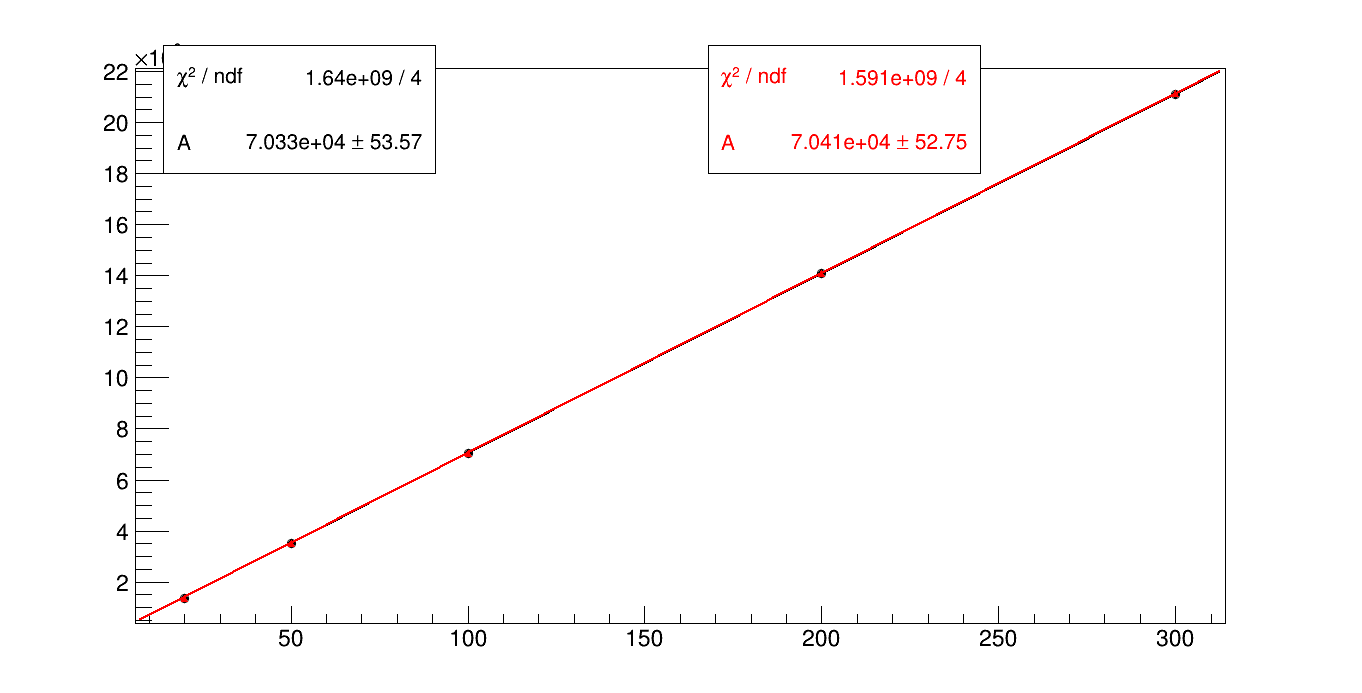
\includegraphics[width=0.95\textwidth]{figures/ch_simulations/he/performance/Linearity.png}
    \caption{The linearity graph of the Shashlik electromagnetic calorimeter (Top) and Hadron Endcap (Bottom). G4Scintillation (Black) and Parametrized (Red). Shows the dependence of the response of the calorimeter as a function of the energy of the incident particle: electron (Shashlik) and pion (Hadron Endcap).}
    \label{fig:simulations_shashlik_linearity}
 \end{figure}

Figures \ref{fig:simulations_shashlik_energyreco}, \ref{fig:simulations_he_energyreco} show the reconstructed energy distributions for Shashlik and HE, respectively. Shashlik and HE are calibrated separately as they constitute isolated parts of the system. Note this is different with respect to HGC, where calibration of EM and FH parts was done together. The energy reconstruction is obtained by applying the Calibration Coefficient (CC) that converts the number of optical photons generated to the actual units of energy.
\begin{figure}[hbtp]
    \centering
    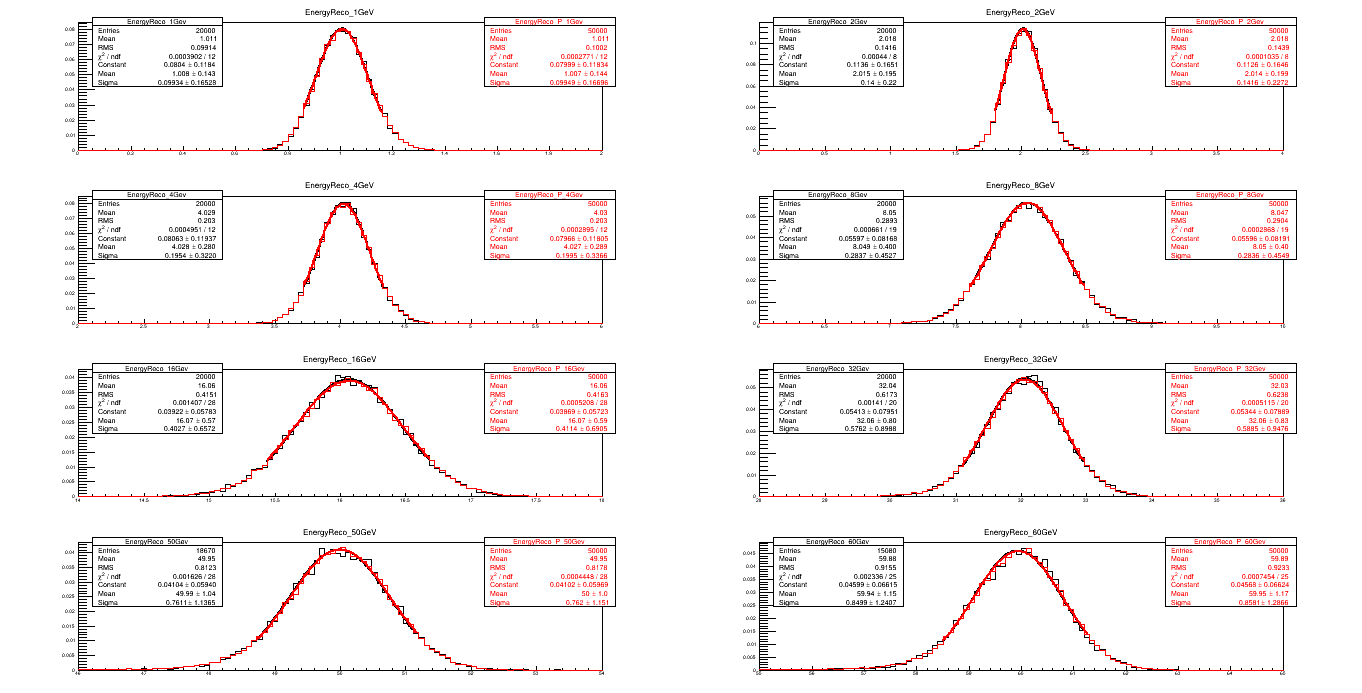
\includegraphics[width=0.95\textwidth]{figures/ch_simulations/shashlik/performance/EnergyRecoDistributions.png}
    \caption{Reconstructed Energy Distributions for Shashlik. G4Scintillation (Black) and Parametrized (Red). Electron particle gun used with eight different energies: 1 GeV, 2 GeV, 4 GeV, 8 GeV, 16 GeV, 32 GeV, 50 GeV and 60 GeV.}
    \label{fig:simulations_shashlik_energyreco}
 \end{figure}
 \begin{figure}[hbtp]
    \centering
    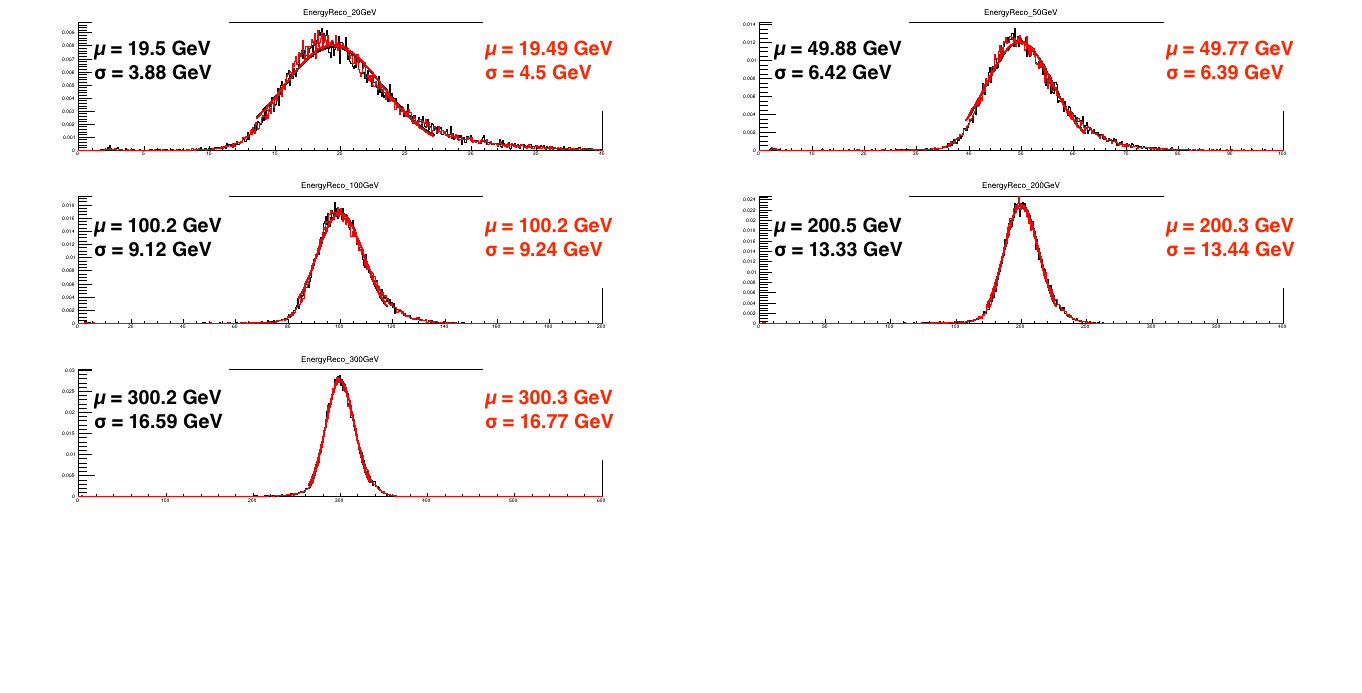
\includegraphics[width=0.95\textwidth]{figures/ch_simulations/he/performance/EnergyRECODistributions.png}
    \caption{Reconstructed Energy Distributions for Hadron Endcap. G4Scintillation (Black) and Parametrized (Red). Pion particle gun used with five different energies:  20 GeV, 50 GeV, 100 GeV, 200 GeV, 300 GeV.}
    \label{fig:simulations_he_energyreco}
 \end{figure}

 Results for the energy resolution are provided in Figure \ref{fig:simulations_shashlikhe_resolution}. The differences between the parametrized response and the use of optical photons are negligible.
 \begin{figure}[htbp]
    \centering
    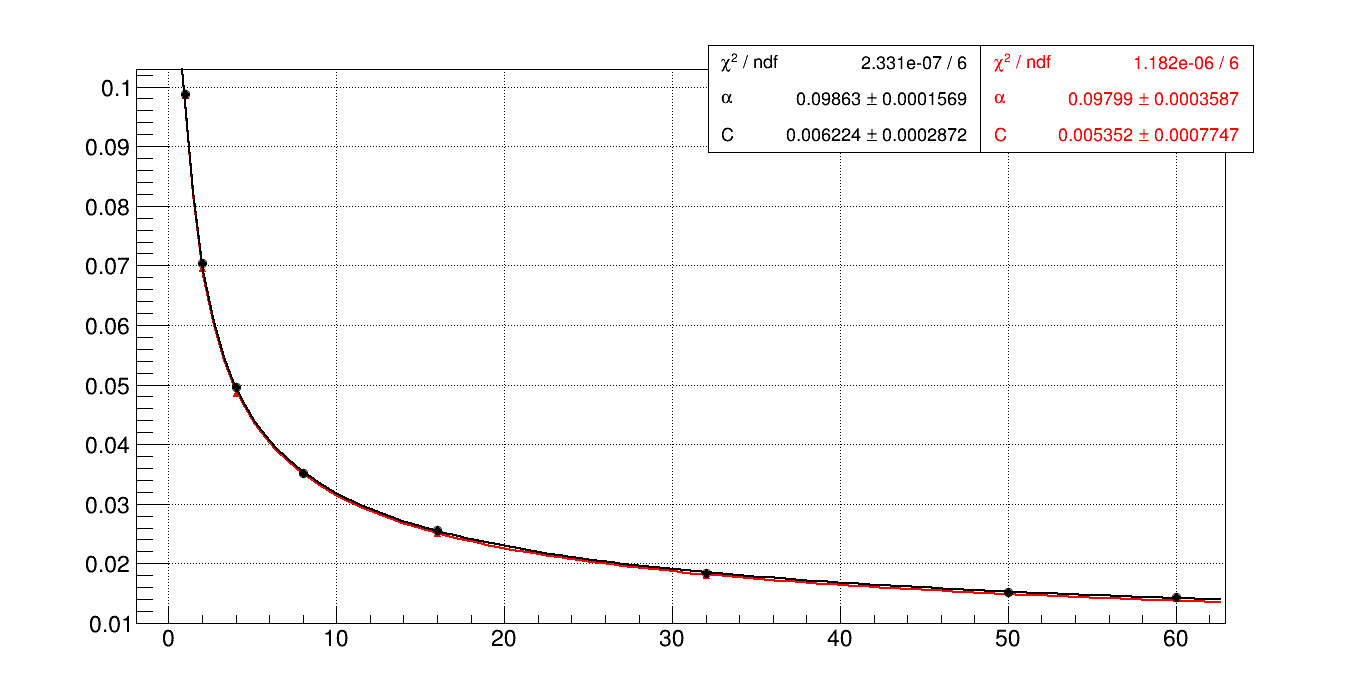
\includegraphics[width=0.95\textwidth]{figures/ch_simulations/shashlik/performance/energyResolution.png}\\
    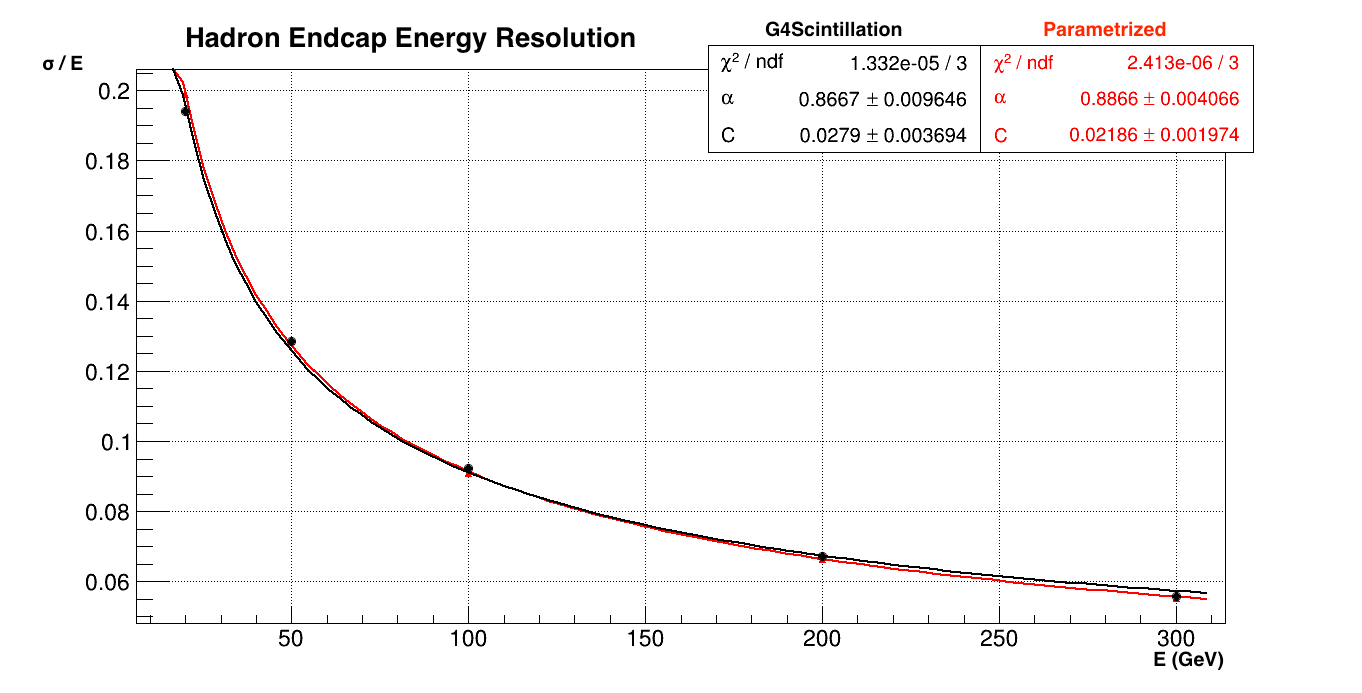
\includegraphics[width=0.95\textwidth]{figures/ch_simulations/he/performance/Resolution.png}
    \caption{Energy Resolution for Shashlik (Top) and for Hadron Endcap (Bottom). G4Scintillation (Black) and Parametrized (Red). For the Shashlik system, the stochastic component $\alpha$ ($\approx 0.01$) determines the level of statistical fluctuations and C (0.6\%) shows the behavior of the system at high energies. Similarly, for the Hadron Endcap, the stochastic component $\alpha$ is $\approx 0.87$ and C is $\approx0.03\%$.}
    \label{fig:simulations_shashlikhe_resolution}
 \end{figure}